\documentclass{article}
\usepackage{amsmath}
\usepackage{amsthm}
\usepackage{amssymb}
\usepackage{hyperref}
\usepackage[style=apa]{biblatex}
\usepackage[shortlabels]{enumitem}
\usepackage{graphicx}
\bibliography{sources.bib}

\newtheorem{theorem}{Theorem}[subsection]
\newtheorem{corollary}{Corollary}[subsection]
\newtheorem{lemma}{Lemma}[subsection]
\theoremstyle{definition}
\newtheorem{definition}{Definition}[subsection]

\title{Prospectus DRAFT}
\author{Connor Hanley}
\date{\today}

\begin{document}
\maketitle

\begin{abstract}
  Dense Associative Memories generalize traditional Hopfield networks, and
  provide a mechanism to drastically improve their theoretical storage
  capacity. To do this, they perform a non-linear operation on the
  similarities between cue or query patterns with memorized patterns. These
  improvements come at the cost of the simple intuitions of Hopfield networks.
  We discuss contemporary and historical research in the field, and provide
  desiderata for a Hebbian model which retains the intuition and
  simplicity of Hopfield networks, without sacrificing theoretical storage
  capacity.
\end{abstract}

\section{Introduction}

Humans are able to recognize and retrieve patterns of data using distorted,
noisy, and partial patterns \parencite{rumelhart_general_1986}. This
capacity of human memory is known as \textit{content-addressability}: patterns
which are stored in memory are able to be ``looked up'' by themselves or their
parts. Modeling this property is a classical task in computational cognitive
and neuroscience (see \textcites{marr_simple_1971,little_existence_1974,
amari_learning_1972,nakano_associatron-model_1972,stanley_simulation_1976}).
The family of models which implement content-addressability are known
as \textit{associative memory models} (AMs). AMs are able to account for many
cognitive tasks, (INSERT EXAMPLES HERE) \parencite{hintzman_minerva_1984}.
A recent revival of interest AMs in machine learning research,
driven by their equivalence with ``attention'' layers in the transformer
architecture \parencites{vaswani_attention_2023, ramsauer_hopfield_2021},
has led to drastic advances in the storage capacity of AMs
\parencites{demircigil_model_2017,krotov_dense_2016,hu_provably_2024}.

Traditional models of Associative Memory rely on Hebbian update rules
to memorize stored patterns in the weights of lateral connections
\parencites{amari_learning_1972,hopfield_neural_1982,kohonen_correlation_1988,
nakano_associatron-model_1972}. Hebbian update rules are appealing
for cognitive
and neuroscience as the weight updates are both entirely \textit{local} and
the representation of content is \textit{distributed}. By local, we mean
that the interactions between artificial neurons are entirely defined by
local connections between other neurons. By distributed content, we mean that
the representations of features, stimuli, and patterns are not defined in terms
of single memory locations (like conventional digital computers), but rather
are represented in the interactions over many artificial neurons (for motivation
see \textcite{mcclelland_appeal_1986}).

While traditional models have desirable properties, they suffer from small
storage capacities \parencites{hopfield_neural_1982,amit_storing_1985},
scaling linearly with the dimension of patterns stored. Dense
Associative Memories have generalized traditional models, providing a
theoretical
storage capacity which scales exponentially with the dimension of the patterns
stored \parencites{krotov_dense_2016,demircigil_model_2017}. This discovery
has been incredibly fruitful, leading to increased interpretability of
large language models based on the Transformer architecture
\parencites{vaswani_attention_2023,ramsauer_hopfield_2021}, as well as the shift
from memorization to generalization in modern deep learning architectures
\parencite{pham_memorization_2025}. However, in spite of these gains,
the Hebbian
intuition and plausibility is lost \parencite{mcalister_sequential_2025}.
Instead of relying on local update rules, Dense Associative Memories
train using back-propagation of error.

%% I think that holographic memories are out of scope, but should be conisdered
%% they're not necessarily hebbian ? I need to think about that : and it would
%% be fruitful to include them in rigorous testing of the memories either way
In the following, we will investigate what a Hebbian alternative to Dense
Associative Memory must look like in order to maintain biological plausibility
and inherent interpretability without sacrificing theoretical
capacity. To begin,
we will review traditional Associative Memory models, starting with
models similar to or based on Hopfield networks
\parencite{hopfield_neural_1982}.
After, we will review Dense Associative Memory, which generalizes on Hopfield
networks and improves their capacity, with the loss of Hebbian weight updates.
We will then review holographic associative memory models, which are
similarly local (INSERT RESEARCH INTO HOLOGRAPHIC MEMORY HERE).

\section{Background}

\begin{quote}
  ``Men make their own history, but they do not make it as they please; they
  do not make it under self-selected circumstances, but under circumstances
  existing already, given and transmitted from the past. The tradition of all
  dead generations weighs like a nightmare on the brains of the living.''
  \parencite{marx_eighteenth_1852}
\end{quote}

Dense Associative Memories build on a vast wealth of previous research, and
while the desire for a simple and intuitive network which mirrors its qualities
is straightforward, understanding how we get to this point requires
an explanation of the thinking that got to where we are now. In this section
we will detail the background information necessary for understanding Dense
Associative Memories. To begin, we will discuss traditional Associative Memory
models in~\autoref{sec:trad-assc}; next, we will discuss Correlation Matrix
Associative Memories in~\autoref{sec:correl}, which are the framework behind
Hopfield networks, discussed in~\autoref{sec:hopfield}. We will then discuss
the theoretical capacity of Hopfield networks in~\autoref{sec:hopfield-cap}.
Next we will discuss the theory behind Dense Associative Memories, and the
energy-based framework developed behind them in~\autoref{sec:dam}
and~\autoref{sec:uhn}. We will discuss their capacity as well
in~\autoref{sec:dam-cap}. After, we will discuss local Hebbian learning,
the theory behind the simplicity of Hopfield networks in~\autoref{sec:hebb}
and~\autoref{sec:general-hebb}. Finally, we will discuss related associative
memory research: Holographic Associative Memories in~\autoref{sec:ham},~
\autoref{sec:hrr}, and~\autoref{sec:ham-cap}. Finally,

\subsection{Associative Memories}\label{sec:trad-assc}

Associative Memory (AM) models are a family of architectures designed to
learn to associate tuples of patterns $(x, y)$ such that one can recover
$y$ from partially distorted, masked, or noisy forms of $x$. In order to
generalize here, the following formal definition suffices:
\begin{definition}[Associative Memories; auto-association;
  hetero-association]\label{def:assoc-memory}
  An \textit{associative memory} is a $3$-tuple $\langle f, A, C \rangle$
  obeying the following properties:
  \begin{enumerate}[(i)]
    \item The \textit{address} matrix $A$ is an $N \times D$ matrix of
      patterns we wish to learn as \textit{cues} or
      \textit{queries};\label{def:assoc:cond1}
    \item The \textit{content} matrix $C$ is an $N \times M$ matrix of
      patterns we wish to learn as \textit{responses}, or associate with
      each $a_i$, $i = 1, 2, \dots, N$; and, \label{def:assoc:cond2}
    \item The \textit{recall} function
      $f_{A, C} : \mathbb{R}^D \to \mathbb{R}^M$ maps $D$-dimensional query or
      cue patterns $x$ to memorized $M$-dimensional patterns $y$.
      \label{def:assoc:cond3}
  \end{enumerate}
  An associative memory $\mathcal{M}$ is said to be \textit{auto-associative}
  iff the address matrix is equivalent to the content matrix, i.e. $A=C$.
  It is sufficient, then, to only specify a recall function and
  address matrix for
  auto-associative memories.  Associative memories are said to be
  \textit{hetero-associative} otherwise.
\end{definition}
Another typical property of AMs is \textit{content-addressability}, which
describes the task of recovering a stored content based on a partial subset
of the information with it's associated query
\parencites{mcclelland_appeal_1986,haykin_neural_2009}. This is in contrast
to other memory models, for example in the C programming language
(INSERT K\&R citation here), where data
is accessed in memory by arbitrary addresses unrelated to the data itself.

AMs also operate with a distinction between
\textit{recall} and \textit{learning}. In recall, we apply the function
$f_{A,C}$ to some $D$-dimensional pattern $x$ to recover its associated
content $\hat y$. This can be done by a single-pass of $x$ through
a neural network implementing $f_{A,C}$, or by asynchronous energy minimization
(see,~\autoref{sec:hopfield}). In the learning phase, the network adjusts
$f_{A,C}$ via a learning algorithm to minimize the difference
between the estimated content associated with a query, $\hat y$, and the desired
associated content, $y$. This can be done via any learning algorithm that we
choose.

AMs are not able to store an infinite amount of patterns. There is a critical
capacity $N^\text{max}$ for AMs
(being the first dimension of the address and content matrices) at which
recall can no longer adequately produce a $\hat y$ which corresponds with
the desired associated pattern $y$. Critical capacity is
influenced by the kind of data being learned. For example, a real-world
dataset like MNIST \parencite{lecun_mnist_2010} contains images which are
highly correlated with one another. High correlation between stored patterns
requires effective AMs to somehow be sensitive to fine-grain differences, which
will be discussed in~\autoref{sec:dam} and~\autoref{sec:uhn}.

\subsection{Correlation Matrix AMs}\label{sec:correl}

Correlation Matrix AMs are a class of auto-associative AMs which learn to
associate bipolar patterns via a correlation matrix of desired
patterns with themselves,
originally presented in
\parencites{kohonen_correlation_1988,amari_learning_1972,
nakano_associatron-model_1972}:
\begin{definition}[Correlation Matrix Associative Memory]\label{def:correl-mem}
  A \textit{Correlation Matrix} associative memory is an auto-associative
  memory $\langle f, \Xi \rangle$, where:
  \begin{enumerate}[(a)]
    \item The $N \times D$ address matrix $\Xi$ contains $N$ patterns $\xi_i$
      of $D$-dimension; and,
    \item the recall function is:
      $$
      f_\Xi (x) = g \left(\Xi^\top \Xi x\right),
      $$
      and $g$ is some function.
  \end{enumerate}
\end{definition}
Correlation Matrix AMs are so-called as they recall values via the correlation
matrix (in the simplest case) $W = \Xi^\top \Xi$. For
\textcite{kohonen_correlation_1988},
$g$ is just the identify function $g (x) = x$. In
\textcites{amari_learning_1972,hopfield_neural_1982},
$g$ is the \textit{signum} function:
$$
\text{sgn} \left[  n \right] =
\begin{cases}
  -1,&~\text{if}~n < 0, \\
  0,&~\text{if}~n = 0, \\
  1,&~\text{if}~n > 0.
\end{cases}
$$
For a difference between the two $g$ functions, see~\autoref{fig:amari-kohonen}.
With a non-linear $g$ function, have a clarified result which is forced to chose
between the bipolar values $\{-1, 1\}$. Whereas, with $g(x) = x$, it becomes
clear that the reconstructed value is a linear combination of the
stored patterns
weighted by their dot product with the query.
\begin{figure}[t]
  \centering
  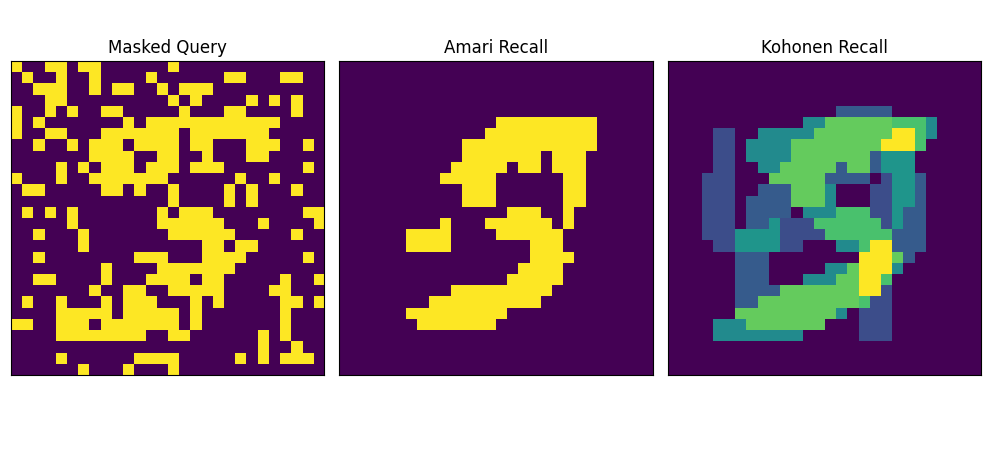
\includegraphics[width=\textwidth]{amari_kohonen_CROPPED.png}
  \caption{Left-to-right: Masked query presented to the networks.
    Single-pass recall
    with $g(x) = \text{sgn}[x]$ (``Amari Recall''). Single-pass recall
  with $g(x) = x$ (``Kohonen Recall'').}
\end{figure}\label{fig:amari-kohonen}
To see how this is the case, suppose that we have pattern matrix $\Xi
= [\xi_1, \xi_2, \dots, \xi_N]$,
and we wish to recall a query pattern $\sigma$. Recall, then, is:
\begin{equation}\label{eq:correl:recall}
  \begin{split}
    f_\Xi (\sigma) &= \Xi^\top \Xi \sigma \\
    &= (\xi_1 \xi_1^\top + \xi_2 \xi_2^\top + \dots + \xi_N
    \xi_N^\top) \sigma \\
    &= (\xi_1 \xi_1^\top \sigma) + (\xi_2 \xi_2^\top \sigma) + \dots
    + (\xi_N \xi_N^\top \sigma) \\
    &= \sum^N_{i=1} \xi_i \left(\xi_i^\top \sigma\right).
  \end{split}
\end{equation}

The structure of \autoref{eq:correl:recall} also shows us how one could simply
learn new representations over a period of time $T = N$. To begin, at
time $t = 0$,
we set the weight matrix $W$ to zeros:
\begin{equation}
  W^{(0)} \gets [0]_{D \times D}.
\end{equation}
At each new time step $t + 1$, we update the weights with the corresponding
pattern we wish to store:
\begin{equation}
  W^{(t+1)} \gets W^{(t)} + \xi_{(t+1)} \xi_{(t+1)}^\top.
\end{equation}
This definition gives us the following \textit{Activity Product Rule}
\parencite{haykin_neural_2009},
\begin{equation}\label{eq:hopfield:apr}
  \Delta W = \xi_i \xi_i^\top.
\end{equation}
We will discuss the Activity Product Rule and other Hebbian learning
rules in~\autoref{sec:hebb}.

\subsection{Hopfield Networks}\label{sec:hopfield}

The main contribution of the work of \textcite{hopfield_neural_1982} is not
the correlation-matrix structure of the associative memory. We have already
discussed the idea of a single layer model with full, lateral connections above
in~\autoref{sec:correl}. Rather, the main contribution of Hopfield was the
introduction of the notion of \textit{energy}, and \textit{energy descent}.
Hopfield networks are characterized by an \textit{energy function},
$E(\sigma^{(t)})$ which
describes the current state of the network. If the energy function
is a Lyapunov function (INSERT DISCUSSION OF LYAPUNOV FUNCTIONS HERE),
and is well-designed, then the local minima of the range of the function
will correspond up to a certain critical capacity with patterns that
we wish the network to store.

More informally, the intuition is that we want to create an ``energy landscape''
via the energy function with dips and divots corresponding to patterns
that we wish to store. ``Energy descent'' is so called because we start with
an initial state of the network, and continuously lower the energy until
it can be no longer lowered. In the same way that a ball set on the incline
of a hill will fall till it reaches the lowest point, so too does an
energy-based
associative memory perform recall.

\begin{definition}[Hopfield network]
  \label{def:hopfield}
  A \textit{Hopfield network} is a single-layer neural network
  which as $D$ computational units with full, lateral connections.
  The state of the $D$ computational units. Let the $N \times D$
  matrix $\Xi = [\xi_1, \xi_2, \dots, \xi_N]$ be the pattern matrix.
  The state of the $D$ computational units, $\sigma^{(t)}$, depends on
  an \textit{energy function}:
  \begin{equation}
    E(\sigma) = - \frac{1}{2} \sum^N_{i=1} (\xi_i \cdot \sigma)^2;
  \end{equation}
  as,
  \begin{equation}
    \sigma_i^{(t+1)} = \arg\min_{b \in \{-1, 1\}} \{ E(\sigma_i^-),
    E(\sigma_i^+) \}
  \end{equation}
  with $\sigma_i^\pm$ being $\sigma^{(t)}$ with the $i$'th element
  multiplied by $\pm 1$ ($b$).
\end{definition}

We can in fact directly demonstrate that Hopfield networks are
approximately equivalent
to Correlation Matrix AMs. This proof is essential for understanding later
developments in the theory of AMs in the same family as Hopfield
networks, and will be
discussed in \autoref{sec:dam}.
\begin{theorem}[Hopfield networks are Correlation Matrix AMs]
  Let us have $D$ computational units $\sigma$ and $N \times D$
  pattern matrix. Then, updating all elements $\sigma_i$, $i = 1,2,\dots D$
  of the state vector by flipping their bit and keeping it if it lowers the
  energy is approximately equivalent to the single-pass update rule of
  correlation matrix AMs.
\end{theorem}

Derivation and intuition come from \textcite{krotov_modern_2025}.
Recall that by Definition~\ref{def:hopfield} the one-step update rule of a
single random bit is:
\begin{equation}\label{proof:random-update}
  \sigma_i^{(t+1)} = \arg\min_{b \in \{-1, 1\}} \{ E(\sigma_i^-),
  E(\sigma_i^+) \}
\end{equation}
Let $F_n (\cdot) = \frac{1}{n} (\cdot)^n$, so $F_2 = \frac{1}{2} (\cdot)^2$.
With $F_2$, we can reformulate the energy function of a Hopfield network as:
\begin{equation}\label{hopfield:f_n}
  E(\sigma) = \sum^N_{i=1} F_2 (\xi_i \cdot \sigma).
\end{equation}
By \textcite{krotov_modern_2025}, we can make a single pass update rule:
\begin{equation}\label{eq:krotov-energy-deriv}
  \forall i \in \{1, \dots, D\},~\sigma_i^{(t+1)} \approx
  \text{sgn} \left[ \sum^N_{j=1} \xi_{ji} F_2' \left( \xi_j \cdot
  \sigma^{(t)}  \right) \right],
\end{equation}
or,
\begin{equation}
  \sigma^{(t+1)} = f_\Xi (\sigma^{(t)}) = \text{sgn} \left[ \Xi^T
  \Xi \sigma^{(t)} \right],
\end{equation}
with $\Xi = [\xi_1, \xi_2, \dots, \xi_N]$.
This is just the single-pass update rule from Definition~\ref{def:correl-mem}
using the \textit{signum} function for $g$.

\subsection{Hopfield Network Capacity}\label{sec:hopfield-cap}

While the simplicity and appeal of Hopfield networks is clear, there
is a problem
for their plausibility as a computational model of the mechanisms for memory in
the brain. Namely, their limited capacity, with the famous result from
\textcite{hopfield_neural_1982} that the critical capacity of patterns
that the network can reliably retrieve is around 15 per cent of the
number of computational
units of the network. Of relevance for our discussion is how we can
systematically
arrive at a critical capacity estimate for any associative memory. Therefore,
here we will see how one can arrive at the capacity result for
Hopfield networks.

The critical capacity of a Hopfield network can be arrived at by deriving
an upper bound on the number of patterns that the network can store while
still having that any pattern stored in the network will be recalled
with minimal
errors \parencites{krotov_dense_2016,demircigil_model_2017,krotov_modern_2025}.
More formally, let $\Xi = [\xi_1, \dots, \xi_N]$ be the set of
$D$-dimensional desired
patterns that we wish for the network to store, and let $\sigma$ be the
$D$-dimensional vector representing the current state of the network
at time $t$.
Then, we initialize $\sigma^{(t=0)}$ to some pattern $\xi_i$, and let the
network evolve. If $\sigma^{(t+1)}$ is roughly equivalent to $\sigma^{(t=0)}$
(w.r.t. some distance function $d(\sigma^{(t+1)}, \sigma^{(t=0)}) >
  \epsilon$, where $\epsilon$
is a constant) then the network is at an energy equilibrium, i.e., a
desired stored pattern.

\subsection{Dense Associative Memories}\label{sec:dam}

Hopfield networks are certainly simple and intuitive. But their strength
is also their weakness: their simplicity leads to low storage capacity,
as we have seen above. This problem, as well as convergent theoretical
work in the study of associative memories unrelated to Hopfield networks,
found an interesting solution: applying a non-linear function to the
dot product scores between the desired stored patterns $x_i$ and the
query pattern $\sigma$.

Early models that used this technique are: \textsf{Minerva2}
\parencite{hintzman_minerva_1984},
which computes the cosine similarity between the query pattern
and stored patterns, and then sums the rows of the element-wise
product of these weighted similarity scores and our desired patterns.
Similar work investigated energy functions with tensor-based
interaction terms \parencites{psaltis_higher_1988,chen_high_1986},
with a unifying approach found in \textcite{kelly_memory_2017}.

A general theory can be found in \textcite{krotov_dense_2016},
later expanded in \textcites{demircigil_model_2017},
and to arbitrarily sized neural networks in \textcite{krotov_hierarchical_2021}.
\begin{definition}[Dense Associative Memory]
  \textit{Dense Associative Memory} is a generalization of Hopfield networks,
  with $N \times D$ pattern matrix $\Xi = [\xi_1, \xi_2, \dots, \xi_N]$,
  $D$-dimensional state vector $\sigma^{(t)}$, and an energy function
  of the form:
  \begin{equation}
    E(\sigma) = - \sum^N_{i=1} F_n \left( \xi_i \cdot \sigma \right),
  \end{equation}
  where $F_n$ is a \textit{polynomial} function $F_n(\cdot) =
  \frac{1}{n}(\cdot)^{n}$ (of the same form
  as~\autoref{hopfield:f_n}).
\end{definition}

The form of the polynomial function $F_n$ is non-trivial, as it relates
to the single-pass rule, by the fact used in~\autoref{eq:krotov-energy-deriv}.
Namely, the \textit{single-pass} rule uses the derivative of $F_n$, $F_n'$,
as its non-linear function. From this definition immediately
follows the next two corollaries.

\begin{corollary}
  Hopfield networks of the form given in Definition~\ref{def:hopfield}
  are Dense Associative Memories, with polynomial function $F_2$.
\end{corollary}
\noindent
To see why this is the case, note that $\frac{d}{dx} F_2' =
\frac{1}{2}(2) (x)^{2-1} = x$.

\begin{corollary}
  The memory model \textsf{Minerva2} from
  \textcite{hintzman_minerva_1984} is approximately
  a Dense Associative Memory with polynomial function $F_4$.
\end{corollary}
\noindent
With polynomial function $F_4$, the energy function becomes:
\begin{equation}
  E(\sigma) = - \frac{1}{4} \sum^N_{i=1} (\xi_i \cdot \sigma)^4.
\end{equation}
By \textcite{krotov_modern_2025}, the update-rule for $\sigma^{(t+1)}$
is (using the same move as in~\autoref{eq:krotov-energy-deriv}):
\begin{equation}\label{dam:minerva2-update}
  \sigma^{(t+1)}_i = \text{sgn} \left[ \sum^N_{j=1} \xi_{ji} (\xi_j
  \cdot \sigma^{(t)})^3 \right].
\end{equation}
Compare the transmission function of \textsf{Minerva2}:
\begin{equation}\label{minerva2-update}
  \sigma^{(t+1)} = \text{sgn} \left[ \sum^N_{i=1} \xi_i
    \left(\frac{\xi_i^\top \sigma^{(t)}}{\|\xi_i\|
  \|\sigma^{(t)}\|}\right)^3 \right].
\end{equation}
If every $\xi_i$, $i=1, 2, \dots, N$ and $\sigma^{(t)}$ are vectors
of magnitude $1$,
then \autoref{dam:minerva2-update} and \autoref{minerva2-update}
are directly equivalent.

The insights of Dense Associative Memories are not limited to binary vectors,
and have been shown to apply to multi-head attention in transformer networks
\parencites{ramsauer_hopfield_2021,vaswani_attention_2023}.

\begin{theorem}
  Any DAM with polynomial function $F_n$, with $n > 2$, is not Hebbian.
\end{theorem}

We say that an architecture is Hebbian if the connections between
every layer $x_i$ and $x_j$, $i \neq 0$ and $j = i + 1$, is entirely
determined by the prior activity of $x_i$, $x_j$, and the
previous connection
weights between them. But, \textcite{krotov_large_2021} notes that
$n \geq 3$ requires many-body neuron interactions, which are non-Hebbian.

One solution, to be discussed in~\autoref{sec:related-work}, is Neuron-astrocyte
memory \parencite{kozachkov_neuron-astrocyte_2024}. Related work
\parencite{ramsauer_hopfield_2021}

\subsection{Dense Associative Memory Capacity}\label{sec:dam-cap}

\begin{theorem}
  The critical capacity, $N^\text{max}$ of any DAM with polynomial
  function $F_n$ scales proportionally to $D^{n-1}$,
  $$
  N^\text{max} \propto D^{n-1}.
  $$
\end{theorem}

See \textcites{demircigil_model_2017,krotov_dense_2016}.

Previous work talks about the number of connections affecting the number of
memories that are capable of being stored \parencite{little_analytic_1978}.
More concrete proof here, reproduce from
\parencites{krotov_dense_2016,demircigil_model_2017}.
Signal-to-noise estimation.

\subsection{Universal Hopfield Networks}\label{sec:uhn}

\begin{definition}[Universal Hopfield Networks]
  \textit{Universal Hopfield Networks} (UHNs) are a general theory
  of single-pass associative memories, where the recall function $f$
  can be broken into
  three parts:
  $$
  f_{A,C}(\sigma) = \underbrace{C^T}_{\text{Projection}} \left(
    \underbrace{\text{sep}}_{\text{Separation function}}
    \left[ \underbrace{\text{sim}(A, \sigma)}_{\text{Similarity
  function}} \right] \right).
  $$
  Namely:
  \begin{enumerate}[(1)]
    \item A \textit{similarity function}, that computes the relevant
      distance between stored
      patterns and query patterns;
    \item A \textit{separation function}, which is typically
      non-linear, which maximizes
      high similarity values and minimizes low similarity scores; and,
    \item A \textit{projection function}, which generates vectors in the row
      space of the content matrix, formed by the basis vectors of the
      row space of the
      column matrix weighted by their respective separated similarity scores.
  \end{enumerate}
\end{definition}

While investigation into DAMs has revealed that their capacity scales with
the $F_n$, with $F'_n$ being their separation function; informal experimentation
reveals that another important way of increasing capacity is the
similarity function
of the associative memory
\parencites{millidge_predictive_2022,hu_provably_2024}.

\subsection{Hebbian and Local Learning Rules}\label{sec:hebb}

\begin{definition}[Hebbian update]
  A \textit{Hebbian update rule} or \textit{Hebbian learning} rule is an update
  rule which is entirely local. By \textit{local weight update}, we mean that
  the weights connecting layers $x_i$ and $x_j$, $j = i + 1$, are defined
  in terms of: the activity of $x_i$, the activity of $x_j = g(x_i)$, and
  the weights $w_{ij}$:
  \begin{equation}
    \Delta w_{ij} = f (w_{ij}; x_i, x_j).
  \end{equation}
\end{definition}

\begin{definition}[Expanded Hebbian update rule]\label{def:expanded-hebb}
  The \textit{expanded} Hebbian learning rule is the Taylor expansion
  of the weight update rule about $(0, 0)$
  \parencite{gerstner_mathematical_2002}:
  \begin{align*}
    \Delta w_{ij} &= f(w_{ij}; x_i, x_j) \\
    &= f(w_{ij}; 0, 0) + \frac{\partial f}{\partial x_i} \big|_{(0,
    0)} x_i + \frac{\partial f}{\partial x_j}
    \big|_{(0, 0)} x_j \\
    &+ \frac{1}{2} \frac{\partial^2 f}{\partial v^2_i} \big|_{(0, 0)}
    x_i^2 + \frac{1}{2} \frac{\partial^2 f}{\partial v^2_j}\big|_{(0,
    0)} x_j^2 \\
    &+ \frac{\partial^2 f}{\partial x_i \partial x_j}\big|_{(0, 0)}
    x_i x_j + \mathcal{O}(x).
  \end{align*}
  We denote the Taylor coefficients by
  $c_n^{\{\text{corr},~\text{pre},~\text{post}\}}$, with
  $n$ denoting the order of the coefficient, $\text{corr}$ denoting
  the coefficient
  weighting the correlation between the pre- and post-synaptic neural
  layers, and
  $\text{pre}$ and $\text{post}$ to denote the coefficients of the
  pre- and post-synaptic
  layers themselves (respectively).
  This gets us:
  \begin{align*}
    \Delta w_{ij} &= f(w_{ij}; x_i, x_j) =
    c_0 (w_{ij}) + c_1^\text{pre} (w_{ij}) x_j + c_1^\text{post} x_i \\
    &+ c_2^\text{pre} (w_{ij}) x_j^2 + c_2^\text{post} (w_{ij}) x_i^2
    + c_2^\text{corr} (w_{ij}) x_i x_j \\
    &+ \mathcal{O} (x).
  \end{align*}
\end{definition}

\begin{corollary}[Activity Product Rule]
  We can derive the Activity Product Rule in~\autoref{eq:hopfield:apr}
  by setting $c_2^\text{corr}$ to some constant, and letting all other
  coefficients be zero, getting us an update rule:
  $$
  \Delta w_{ij} = c_2^\text{corr} (w_{ij}) x_i x_j.
  $$
  Typically, we denote $c_2^\text{corr} (w_{ij})$ by $\eta$,
  the \textit{learning rate}.
\end{corollary}

%% TODO: fix the notation here: is x_i pre- or post-synaptic neuron?
%% previously we refer to x_i as the pre and x_j as the post, with x_j = g(x_i).
\begin{corollary}[Oja's Rule]
  \textit{Oja's rule} \parencite{oja_simplified_1982} is a competitive Hebbian
  learning algorithm where the weights are naturally normalized. We can
  derive it from Definition~\ref{def:expanded-hebb} by setting
  $c_2^\text{corr} = \eta_0 > 0$,
  and $c_2^\text{post} = - \eta_0 w_{ij}$, with all other
  coefficients set to $0$:
  \begin{align*}
    f(w_{ij}; x_i, x_j) &= \eta_0 x_i x_j - \eta_0 w_{ij} x_i^2 \\
    &= \eta_0 x_i (x_j - w_{ij} x_i).
  \end{align*}
\end{corollary}

\subsection{Related Work}\label{sec:related-work}

\begin{enumerate}[(a)]
  \item Neuron-astrocyte networks
  \item DAM in feature space
  \item Kernel-based DAMS
  \item Predictive Coding Networks
\end{enumerate}

\section{Work Plan}

Completing this project requires two tasks which are interrelated but
practically independent in their execution. The first is the theoretical
work involved in finding a general theory of the capacity of Hebbian
alternatives
to Dense Associative Memories. The second is large-scale experimentation
on real-world datasets We will discuss the theoretical task in
\autoref{subsec:theoretical},
the experimental work in \autoref{subsec:experimental}.

\subsection{Theoretical Work}\label{subsec:theoretical}

Following Definition~\ref{def:expanded-hebb}, we can generate a range of
different Hebbian learning algorithms for a single-layer
network with full lateral connections. All of which are entirely local,
and therefore biologically plausible. There are established methods for
deriving the theoretical capacity of associative memories, as we have
seen in~\autoref{sec:hopfield-cap} and~\autoref{sec:dam-cap}. Therefore,
the goal in this part of the section is to come up with a general theorem
about the critical capacity of associative memories with Hebbian update
rules.
Importantly, the goal here is to provide a parameterized theorem: \textit{how
  do the choices of coefficients in the Expanded Hebbian learning rule
each affect the critical capacity.}

There are two ways of approaching this goal: the first is to ignore
previous Hebbian learning rule research and attack the problem through
permutation of coefficient values. While this approach would be time-consuming,
it would be extensive, and maybe lead to insight from fresh eyes on the problem.
The second way of approaching the problem is to start from extant Hebbian
learning algorithms. Then, we would prove (or find a proof)
for each a critical capacity as a learning rule for an associative memory. This
would be less time-consuming, and provide the project with clearer milestones
and goals. For this approach to be novel, it is not sufficient to just
reiterate the proofs of each update rule's critical capacity. Rather,
after finding or writing each proof, it would be helpful to create a general
theorem for all of them based on common insights.

\subsection{Experimental Work}\label{subsec:experimental}

The second part of the work is experimentation with different Hebbian
learning based associative memories, and comparing their performance to
contemporary models of associative memory. The performance metric by which
to compare each model highly depends on the task. The conventional task
for introducing associative memory models is to do a qualitative evaluation
of their ability to do pattern completion from partially obscured or noisy
queries. While this approach does provide intuitive results, it is hardly
an objective measure beyond broad statements like: the results of
this associative memory ``look'' better than the results of some other.

The second approach for evaluating the performance of associative memories
is to use them for some task as part of a larger network. For example, we can
evaluate the associative memory in a classification task as a part of
a larger network where we input into the network partial or obscured
representations of our domain of interest, and classify the results of the
recall. This latter approach seems to be a better fit for the scientific
evaluation of differing associative memories.

\section{Timeline}

\begin{quote}
  ``The war will be over by Christmas!'' (Many)
\end{quote}

\begin{enumerate}[(a)]
  \item Theoretical investigation by December, paper to follow
  \item Option to either split the experimentation from the theory
    for confirmation as a separate
    paper, or as a single paper
  \item Fitting in Hebbian AMs into Transformer networks; or
    something similar; do they hold
    water to DAMs in sequence prediction/image generation?
  \item Do we see similar memorization $\to$ generalization as DAMs exhibit?
\end{enumerate}

\printbibliography

\end{document}
